\documentclass[12pt, landscape]{article}
\usepackage[scaled=0.92]{helvet}
\usepackage{multicol}
\usepackage{calc}
\usepackage{ifthen}
\usepackage[landscape]{geometry}
%\usepackage{hyperref}

\usepackage{newtxtext} 

%for strikeout
\usepackage{ulem}

%For editing parbox
\usepackage[table]{xcolor}
%For editing itemise margins, reduce item separaion and list separation
\usepackage{enumitem}
\setlist[itemize]{noitemsep}

% For math
\usepackage{amsmath,amsthm,amsfonts,amssymb}

% For justifying
\usepackage{ragged2e}
\justifying

%For pictures / figures
\usepackage{color,graphicx,overpic}
\graphicspath{ {./images/} }

%\usepackage{newtxtext} 
%\usepackage{amssymb}
%\usepackage[table]{xcolor}
%\usepackage{vwcol}
%\usepackage{tikz}
%\usepackage{wrapfig}
%\usepackage{makecell}


% For Code Blocks
\usepackage{xcolor}
\usepackage{listings}



%Helpful:
%[linewidth = 1.0 \linewidth]
%\lstinline{}
% use \code{} for \lstinline with colorbox.
\newcommand{\code}[1]{\colorbox{gray!25!}{\lstinline|#1|}}

\definecolor{dkgreen}{rgb}{0,0.6,0}
\definecolor{gray}{rgb}{0.5,0.5,0.5}
\definecolor{mauve}{rgb}{0.58,0,0.82}
\definecolor{mygray}{rgb}{0.9,0.9,0.9}

\lstset{frame=tb,
  language=SQL,
  aboveskip=1mm,
  belowskip=1mm,
  showstringspaces=false, 
  columns=flexible,
  backgroundcolor=\color{mygray},
  basicstyle={\footnotesize\ttfamily},
  numbers=none,
  numberstyle=\tiny\color{gray},
  keywordstyle=\footnotesize\color{blue},
  commentstyle=\footnotesize\color{dkgreen},
  stringstyle=\footnotesize\color{mauve},
  breaklines=true,
  breakatwhitespace=true,
  tabsize=2
}

% Template: Cheatsheet with code enabled

%--------------------------- PACKAGES ABOVE --------------------------------------------------------------

\pdfinfo{
  /Title (CS2102 Mids Summary.pdf)
  /Creator (Ger Teck)
  /Author (Ger Teck)
  /Subject ()
  /Keywords (tex)}

%% Margins for PAPER

% This sets page margins to .5 inch if using letter paper, and to 1cm
% if using A4 paper. (This probably isn't strictly necessary.)
% If using another size paper, use default 1cm margins.
\ifthenelse{\lengthtest { \paperwidth = 11in}}
	{ \geometry{top=.5in,left=.5in,right=.5in,bottom=.5in} }
	{\ifthenelse{ \lengthtest{ \paperwidth = 297mm}}
		{\geometry{top=1cm,left=1cm,right=1cm,bottom=1cm} }
		{\geometry{top=1cm,left=1cm,right=1cm,bottom=1cm} }
	}

% Turn off header and footer
\pagestyle{empty}

% for tight centres (less spacing)
\newenvironment{tightcenter}{%
  \setlength\topsep{0.5pt}
  \setlength\parskip{0.5pt}
  \begin{center}
}{%
  \end{center}
}

% Redefine section commands to use less space
\makeatletter
\renewcommand{\section}{\@startsection{section}{1}{0mm}%
                                {-1ex plus -.5ex minus -.2ex}%
                                {0.5ex plus .2ex}%x
                                {\normalfont\large\bfseries}}
\renewcommand{\subsection}{\@startsection{subsection}{2}{0.1mm}%
                                {-1explus -.5ex minus -.2ex}%
                                {0.5ex plus .2ex}%
                                {\normalfont\normalsize\bfseries}}
\renewcommand{\subsubsection}{\@startsection{subsubsection}{3}{0.1mm}%
                                {-1ex plus -.5ex minus -.2ex}%
                                {1ex plus .2ex}%
                                {\normalfont\small\bfseries}}
% change font
%\renewcommand{\familydefault}{\sfdefault}
%\renewcommand\rmdefault{\sfdefault}
\linespread{1.05}

\makeatother

% Define BibTeX command
\def\BibTeX{{\rm B\kern-.05em{\sc i\kern-.025em b}\kern-.08em
    T\kern-.1667em\lower.7ex\hbox{E}\kern-.125emX}}

% Don't print section numbers
\setcounter{secnumdepth}{0}

\setlength{\parindent}{0pt}
\setlength{\parskip}{0pt plus 0.5ex}

%% this changes all items (enumerate and itemize, reduce margins)
\setlength{\leftmargini}{0.5cm}
\setlength{\leftmarginii}{0.5cm}
\setlist[itemize,1]{leftmargin=2mm,labelindent=1mm,labelsep=1mm, itemsep = 1mm}
\setlist[itemize,2]{leftmargin=4mm,labelindent=1mm,labelsep=1mm, itemsep = 1mm}
\itemsep = 0mm
\setlist{nosep}

% Need Logo Picture
%Watermark Top Right
%\usepackage{atbegshi,picture}
%\AtBeginShipout{\AtBeginShipoutUpperLeft{%
 % \put(\dimexpr\paperwidth-1.2cm\relax, -1.2cm){\makebox[0pt][r]{\framebox{
\includegraphics[width = 0.3cm]{mountainbooks} Ger Teck}}}%
%}}


% -------------------------------------------------------------------------------

% START OF DOCUMENT HERE

\begin{document}
\raggedright
\footnotesize
\begin{multicols*}{3}



% multicol parameters
% These lengths are set only within the two main columns
%\setlength{\columnseprule}{0.25pt}
\setlength{\premulticols}{1pt}
\setlength{\postmulticols}{1pt}
\setlength{\multicolsep}{1pt}
\setlength{\columnsep}{2pt}

%% DOCUMENT NAME HERE
\begin{center}
     \Large{\textbf{CS2102 Database Sys Summary}} \\
\end{center}

AY23/24 Sem 1, github.com/gerteck
  
\section{Topics \& Objectives}
\justify{
\begin{itemize}
	\item \textbf{Design}: Entity-Relationship (ER) Model, Functional Dependencies, Normal Forms
	\item \textbf{Implementation}: SQL (Data definition language, Queries, Stored procedures, Triggers)
	\item\textbf{Theory}: Relational Calculus and algebra
	\item Module covers fundamental concpets and techniques for:
	\begin{itemize}
		\item Understanding and practice of design \& implementation of database applications and management of data with relational db management systems.
		\item Design of ER data models to capture data requirements, translate to relational database schema, refine using schema decompositions to avoid anomalies.
		\item Use SQL to define relational schemas, write queries.
		\item Reason about correctness using concepts of formal query lang (relational calculus \& algebra) and apply knowledge to develop database applications.	
	\end{itemize}
\end{itemize}
}
\centerline{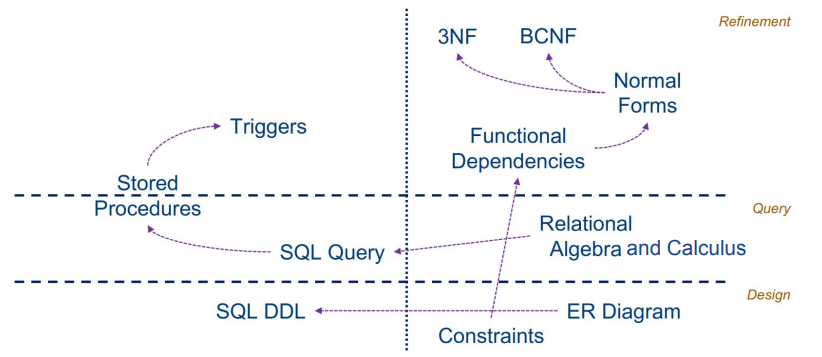
\includegraphics[width=0.9 \linewidth]{roadmap}}

\section{1. Database Management Sys DBMS}
\subsubsection{Challenges for Data-Intensive applications}
\justify{
\begin{itemize}
	\item \textbf{Efficiency}: Fast access to information in volumes of data
	\item \textbf{Transactions}: "All or nothing" changes to data
	\item \textbf{Data Integrity}: Parallel access and changes to data
	\item \textbf{Recovery}: Fast and reliable handling of failures (e.g. HDD/Sys crash, power outage, network disruption)
	\item \textbf{Security}:  Fine-grained data access rights
\end{itemize}
  
\subsubsection{File-based data management to DBMS}
\begin{itemize}
	\item Complex, low level code, Often similar requirements across different programs
	\item \textbf{Problems}:  High development effort, Long development times, Higher risk of (critical) errors
	\item \textbf{DBMS}:  Set off universal and powerful functionalities for data management, with faster application development, higher stability, less errors.
\end{itemize}

\subsubsection{Core concepts of DBMS}
\begin{itemize}
	\item \textbf{ACID Transaction}:  Finite sequence of database operations (reads and/or writes), smallest logical unit of work
	\item \textbf{Atomicity}:  either all effects of T are reflected in the database or none ("all or nothing")
	\item \textbf{Consistency}: the execution of T guarantees to yield a correct state of the database
	\item \textbf{Isolation}:  execution of T is isolated from the effects of concurrent transactions
	\item \textbf{Durability}: after commit of T, its effects are permanent even in case of failures 
\end{itemize}

\subsubsection{Concurrent Execution}
\centerline{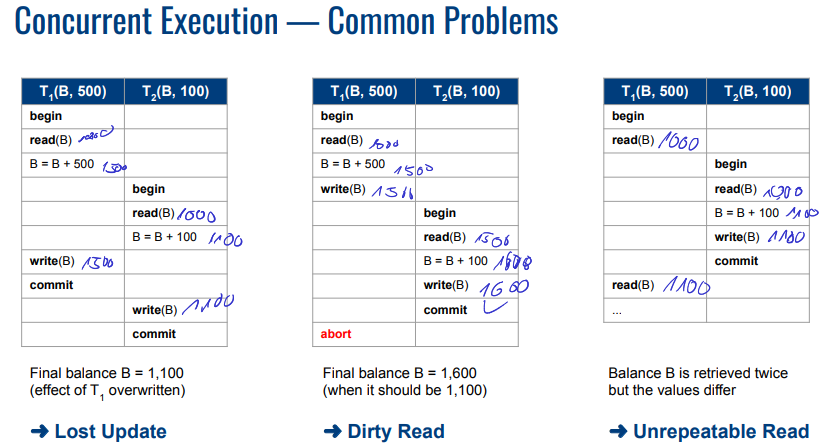
\includegraphics[width=0.7 \linewidth]{concurrentproblems}}
Require Serializable transaction execution:
\begin{itemize}
	\item A concurrent execution of a set of transactions is serializable if this execution 
	is equivalent to some serial execution of the same set of transactions
	\item Two executions are equivalent if they have the same effect on the data
	\item \textbf{DBMS}: Support concurrent executions of transactions to optimize performance, Enforce serializability of concurrent executions to ensure integrity of data
\end{itemize}
}

\subsubsection{Data Abstraction}
\centerline{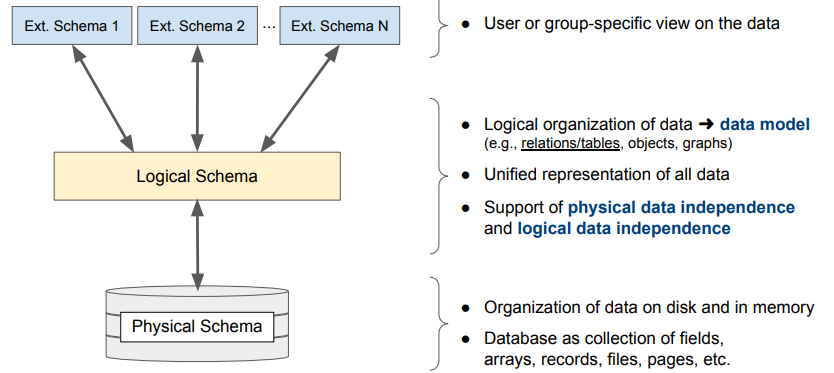
\includegraphics[width=0.9 \linewidth]{dataabstraction}}
\subsubsection{Data Independence}
\centerline{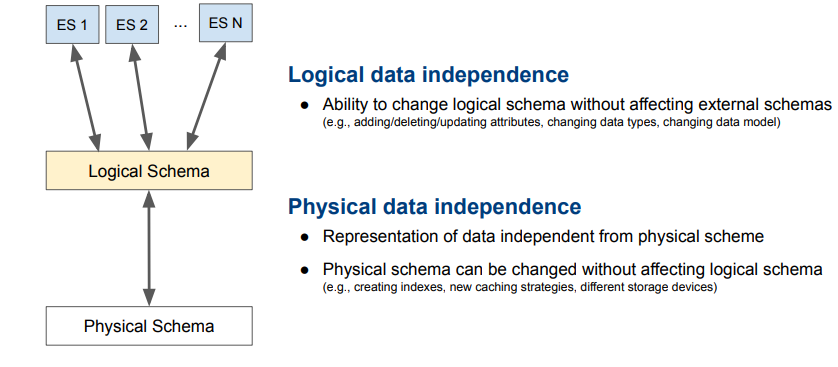
\includegraphics[width=0.9 \linewidth]{dataindependence}}

\justify{
\subsection{Terminology / Definitions}
\begin{itemize}
	\item \textbf{Data Model}: Collection of concepts for describing data
	\item \textbf{Schema}: Description of structure of DB using data model
	\item \textbf{Schema Instance}: Content of a DB at a particular time
\end{itemize}
\subsubsection{Relational Data Model}
Data is modelled by relations, and each relation has a definition called a relation schema. This schema specifies attributes (columns) and data constrains (e.g. domain constraints)
\begin{itemize}
	\item \textbf{Relation}: Can be seen as Tables with rows and columns:
	\begin{itemize}
		\item No. of cols = Degree/Arity, No. of rows = Cardinality
		\item Each row is called a tuple/record. It has a component for each attribute of the relation.
		\item A relation is thus a set of tuples and an instance of the relation schema, i.e. of a single table.
	\end{itemize}
	\item \textbf{Domain}: Set of atomic values, e.g. integers. All values for an attribute is either in this domain or null.
	\item \textbf{Relational database schema}: Set of relation schemas and their data constraints, i.e. of multiple tables
	\item \textbf{Relational database}:  Instance of the schema and is a collection of tables.
\end{itemize}
\centerline{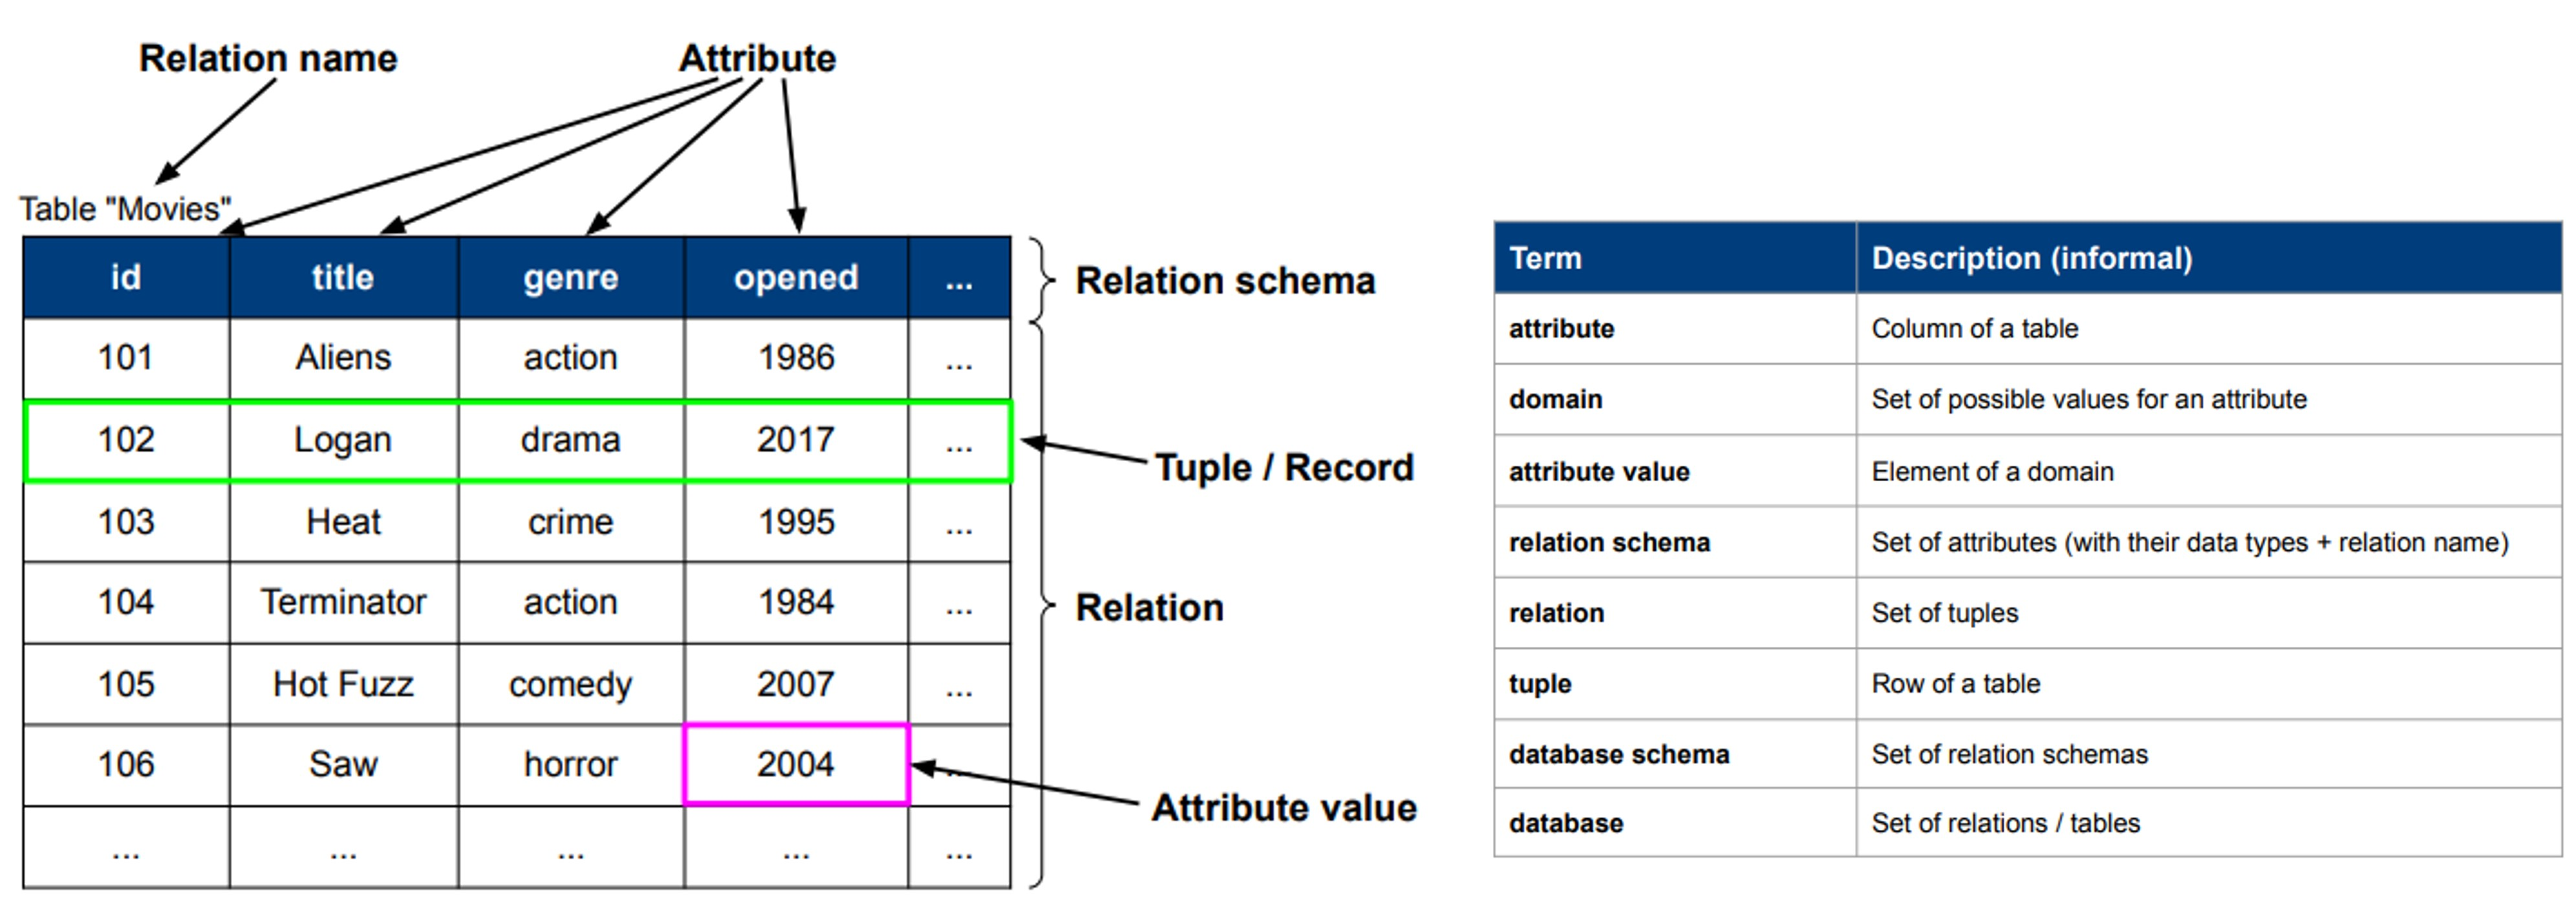
\includegraphics[width=1 \linewidth]{relationalterms}}

\subsection{Integrity Constraints}
Condition that restricts the data that can be stored in a database instance. A legal relation instance is a relation that satisfies all specified ICs.
\begin{itemize}
	\item \textbf{Domain Constraints}:  Restrict the attribute values of relations, e.g. only integers allowed
	\item \textbf{Key Constraints}:
	\begin{itemize}
		\item \textbf{Superkey}: A superkey is a subset of attributes in a relation that unique identifies its tuples.
		\item \textbf{Key}:  A key is a superkey which is minimal, i.e. no proper subset of itself is a superkey. 
		\item \textbf{Candidate keys}: Set of all possible keys for a relation. One of these keys is selected as the primary key.
		\item \textbf{Primary key}: Chosen candidate key for a relation, Cannot be null (entity integrity constraint), Underlined in relation schema. Prime attribute: Attribute of a primary key (cannot be null)
	\end{itemize}
	\item \textbf{Foreign Key Constraints}:
	\begin{itemize}
		\item \textbf{Foreign key}:   A foreign key refers to the primary key of a second relation (which can be itself)
		\item Each foreign key value must be the primary key value in the referenced relation or be null (foreign key constraint)
		\item  Also known as referential integrity constraints.
	\end{itemize}
\end{itemize}
\centerline{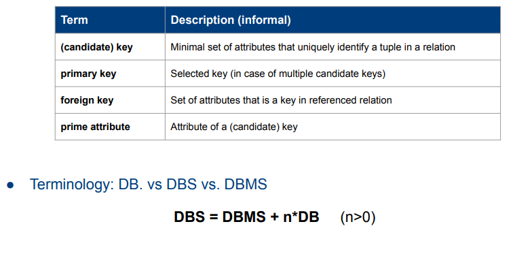
\includegraphics[width=0.8 \linewidth]{integrityconstraints}}
}

\section{2. SQL: Structured Query Language}
\begin{itemize}
\item  Declarative language: focus on what to compute, not on how to compute
\item Contains two parts: Data Definition Language and Data Manipulation Language
\end{itemize}
\subsubsection{Datatypes}
\centerline{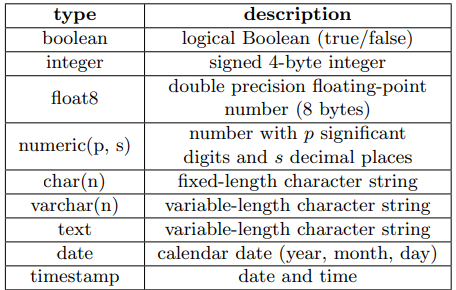
\includegraphics[width=0.6 \linewidth]{datatypes}}

\subsection{Integrity Constraints 2}
\begin{itemize}
	\item A \textbf{consistent state} of the database is a state which complies with the with the business
		rules as defined by the structural constraints and the integrity constraints in the schema.
	\item If an integrity constraint is violated by an operation or a transaction, the operation or the transaction is aborted and rolled back and its changes are undone, otherwise, it is
		committed and its changes are effective for all users.
	\item Five main kinds of integrity constraints in SQL: \textbf{ NOT NULL, PRIMARY KEY, UNIQUE, FOREIGN KEY, CHECK.}
\end{itemize}
\subsubsection{Primary Key}
A primary key is a set of columns that uniquely identifies a record in the table. Each table has at most one primary key. The primary key can be one column or a combination of columns.

\begin{lstlisting}
-- Declare primary key as column constraint
CREATE TABLE customers (
 firstname VARCHAR(64  ,
 lastname VARCHAR(64) ,
 email VARCHAR(64) ,
id VARCHAR(16) PRIMARY KEY);
\end{lstlisting}
\subsubsection{Composite Primary Key \& NOT NULL }
A not null constraint guarantees that no value of the column can be set to null. A not null constraint is always declared as a row constraint. When it is explicit, it is declared with the keyword NOT NULL.
\begin{lstlisting}
CREATE TABLE games (
name VARCHAR(32) ,
version CHAR(3) ,
price NUMERIC NOT NULL,
PRIMARY KEY (name, version) );
\end{lstlisting}

\subsubsection{Data Insertion \ Populating Tables}
\begin{lstlisting}
INSERT INTO customers VALUES(
'Carole', 'Yoga', 'cyoga@email.org',
'Carole89');
\end{lstlisting}

\subsubsection{Deleting Tables}
\begin{lstlisting}
DELETE FROM customers
-- DROP deletes content \& table definition
DROP TABLE customers 
DROP TABLE IF EXISTS downloads  
\end{lstlisting}

\subsubsection{Unique}
A unique constraint on a column or a combination of columns guarantees the table cannot contain two records with the same value in the corresponding column or combination of columns.
\begin{lstlisting}
CREATE TABLE customers (
firstname VARCHAR(64) NOT NULL ,
lastname VARCHAR(64) NOT NULL,
email VARCHAR(64) UNIQUE NOT NULL,
id VARCHAR(16) PRIMARY KEY,
UNIQUE (firstname, lastname));
\end{lstlisting}

\subsubsection{Foreign Key}
\begin{itemize}
\item A foreign key constraint enforces \textbf{referential integrity}. The values in the columns for which the constraint is declared must exists in the corresponding columns of the referenced table.
\item Referenced columns are usually required to be the primary key of the referenced table. Some systems relax this.
\item A foreign key is declared using the keyword REFERENCES as a row constraint and the keywords FOREIGN KEY and REFERENCES as a table constraint.
\end{itemize}
\begin{lstlisting}
CREATE TABLE downloads (
customerid VARCHAR (16) REFERENCES customers (id),
name VARCHAR (32)
version CHAR (3),
FOREIGN KEY ( name, version) REFERENCES games (name, version) );
\end{lstlisting}

\subsubsection{Check}
\begin{itemize}
\item Check constraint enforces any other condition that can be expressed in SQL. Declared as row or table constraint. 
\end{itemize}
\begin{lstlisting}
CREATE TABLE games (
name VARCHAR(32),
version CHAR(3),
PRIMARY KEY (name, version)
price NUMERIC NOT NULL CHECK (price > 0)
-- or as table constraint:
CHECK (price > 0) );
\end{lstlisting}

\subsubsection{Update and Delete Propagation}
\begin{itemize}
\item The annotations ON UPDATE/DELETE with the option CASCADE propagate the update or deletion, when there are chains of foreign key dependencies.
\end{itemize}
\begin{lstlisting}
CREATE TABLE downloads(
id VARCHAR (16) REFERENCES customers (id)
	ON UPDATE CASCADE
	ON DELETE CASCADE,
name VARCHAR(32),
version CHAR(3),
PRIMARY KEY (id, name, version),
FOREIGN KEY (name, version) REFERENCES games(name, version)
	ON UPDATE CASCADE
	ON DELETE CASCADE);
\end{lstlisting}

\begin{itemize}
\item Generally a good idea to constraint all columns not to be null unless there is a good design or tuning reason for not doing so.
\item Think carefully about which foreign keys should be subject to cascade.
\item  Good idea to defer all the constraints that can be deferred. These are checked at the end of a transaction and not immediately after each.
operation.
\end{itemize}

\subsection{Querying Tables}
\subsubsection{Print Table}
• Wildcard '*' to include all attributes
\begin{lstlisting}
SELECT *
FROM customers;
\end{lstlisting}
\subsubsection{View}
	\begin{itemize}
		\item We can give a name to a query, called a view. Once created, a view can be queried like a table.
		\item Creating a view is generally a better option than creating and populating a table,
		temporary or not.
	\end{itemize}
\begin{lstlisting}
CREATE VIEW sg\_customers AS
SELECT  c.firstname, c.lastname, c.email, c.id
FROM customers c
WHERE country = 'Singapore';
\end{lstlisting}
\begin{lstlisting}
SELECT * FROM sg\_customers;
\end{lstlisting}



\section{3. SQL Queries}
\subsubsection{Printing one Table}
\begin{lstlisting}
SELECT firstname, lastname
FROM customers
WHERE country = 'Singapore';
\end{lstlisting}
\subsubsection{DISTINCT and ORDER BY}
• Selecting a subset of columns may result in duplicate row even if original table has a primary key. \\
• DISTINCT keyword eliminates eventual duplicates, requests results contain distinct rows. \\
• Both DISTINCT and ORDER BY involve sorting and conceptually ORDER BY is applied before SELECT DISTINCT.
\begin{lstlisting}
SELECT DISTINCT name, version 
FROM downloads
ORDER BY name ASC, version DESC;
\end{lstlisting}

\subsubsection{WHERE}
• Returns rows that evaluate to true, filter rows on a Boolean condition \\
• Uses Boolean operators such as AND, OR and NOT, and various comparison operators such as \code{>, <, >=, <=, <>, IN, LIKE} and \code{BETWEEN AND} \\
• Does not return rows that evaluate to unknown/null! \\
• '-' matches single char \\
• '\%' matches any sequence of zero or more chars
\begin{lstlisting}
SELECT firstname, lastname
FROM customers
WHERE country IN ('Singapore', 'Indonesia')
AND (dob BETWEEN '2001-01-01' AND '2000-12-01' OR since >= '2016-12-01 )
AND lastname LIKE 'B%'
\end{lstlisting}
• PostgreSQL use "||" for concatenation 
\begin{lstlisting}
-- Not to collect GST below 30 cents:
SELECT name || ' ' || version AS game, price * 1.07
FROM games
WHERE price * 0.07 < 0.3
\end{lstlisting}

\subsubsection{De Morgan's Laws}
\begin{lstlisting}
SELECT name 
FROM games
-- all 3 are the same:
WHERE (version = '1.0' or version = '1.1')
WHERE version IN ('1.0', '1.1')
WHERE NOT (version <> '1.0' AND version <> '1.1');
\end{lstlisting}
  
\subsubsection{NULL value}
• Every domain has additional value, null. Ambiguous, could be ”unknown”, ”does not exists”, or both. In SQL it is generally (but not always) ”unknown”. \\
• With null values, the logic of SQL is a three valued logic with unknown. \\
• Use \code{IS (NOT) NULL} for comparison with null
• \code{COALESCE()} returns the first non-null of its argument.
• \code{COUNT(*)} counts NULL values. \code{COUNT(att) AVG(att) MAX(att) MIN(att)} eliminate null values

\subsubsection{Cross Join}
• Cross join \& Cartesian Product \& cross product, represented by comma \code{CROSS JOIN} \code{,} \\
• Cross join with \code{WHERE} clause: add condition that FK columns equal to the corresponding PK columns. \\
• Systematically define table variables (e.g. \code{games AS g})
\begin{lstlisting}
SELECT *
FROM customers c, downloads d, games g
WHERE d.id = c.id
AND d.name = g.name
AND d.version = g.version
\end{lstlisting}

\section{4. Algebraic SQL Queries}
\subsubsection{Inner Join}
• \code{JOIN} interpreted as \code{INNER JOIN} 
• Inner joins combine records from two tables whenever there are matching values in a field common to both tables.
\begin{lstlisting}
SELECT *
FROM customers c JOIN downloads d ON d.id = c.id
JOIN games g ON d.name = g.name AND d.version = g.version;
\end{lstlisting}

\subsubsection{Natural Join}
•  If we give the same name to columns that are the same, can use natural join. Joins the rows that have the same values for their columns that have the same names. It also prints one of the two equated columns
\begin{lstlisting}
SELECT *
FROM customers c NATURAL JOIN downloads d NATURAL JOIN games g;
\end{lstlisting}

\subsubsection{Outer Join}
• outer join keeps the columns of the rows in the left (left outer join), right (right outer join) or in both (full outer join) tables that do not match anything in the other
table according to the join condition and pad the remaining columns with null values. \\
• Better to avoid outer joins whenever possible as they introduce null values. \\
• \code{RIGHT (OUTER) JOIN, LEFT (OUTER) JOIN} \\
• \code{ FULL (OUTER) JOIN} 
\begin{lstlisting}
-- finds customers, never downloaded a game
SELECT c.id FROM customers c 
LEFT JOIN downloads d ON c.id = d.id
WHERE d.id IS NULL;
\end{lstlisting}

\subsubsection{Set Operations}
• Union, intersect and non-symmetric difference. \\
• Eliminate duplicates: \code{UNION, INTERSECT, EXCEPT} \\
• Keep duplicates: \code{UNION ALL, INTERSECT ALL} \\
\code{EXCEPT ALL}

\section{4. Aggregate SQL Queries}
\subsubsection{Aggregate Functions}
• The values of a column can be aggregated aggregation functions such as \code{COUNT(), SUM(), MAX(), MIN()} \\
\code{AVG(), STDDEV()} etc.
\begin{lstlisting}
SELECT COUNT(*) 
FROM customers c;
\end{lstlisting}

\begin{lstlisting}
-- ALL is default and omitted
-- DISTINCT needed 
SELECT COUNT(ALL DISTINCT c.country) 
FROM customers c;
\end{lstlisting}

\begin{lstlisting}
-- Finds min, max, avg and stddev, TRUNC() displays 2 d p
SELECT MAX(g.price),
MIN(g.price),
TRUNC(AVG(g.price), 2) AS ave,
TRUNC(STDDEV(g.price), 2) AS std
FROM games g;
\end{lstlisting}

\subsubsection{Group By}
• The GROUP BY clause creates groups of records that have the same values for the
specified fields before computing the aggregate functions. \\
• Groups are formed after the rows have been filtered by the WHERE clause \\
• Recommended (and required by SQL standard) to include attributes projected in the SELECT clause in the GROUP BY clause. \\
• The order of columns in the GROUP BY clause does not change the meaning of the query.
\begin{lstlisting}
SELECT c.country, COUNT(*)
FROM customers c
WHERE c.dob >= '2000-01-01'
GROUP BY c.country
\end{lstlisting}

\begin{lstlisting}
SELECT c.country, EXTRACT( YEAR FROM c.since) AS regyear, COUNT(*) AS total
FROM customers c, downloads d
WHERE c.id = d.id
GROUP BY c.country, regyear,
ORDERBY regyear, c.country;
\end{lstlisting}

\subsubsection{Having}
• Aggregate functions can be used in conditions. However, agg. functions not allowed in WHERE. \\
• \code{HAVING} clause to add conditions to be checked after the evaluation of the GROUP BY. \\
• \code{HAVING} can only involve aggregate functions, columns listed in the GROUP BY clause and subqueries.

\begin{lstlisting}
SELECT c.country, 
FROM customers c
GROUP BY c.country
HAVING COUNT(*) >= 100;
\end{lstlisting}

\section{5. Nested SQL Queries}
\subsubsection{Subqueries}
• In FROM clause: Must be enclosed in parenthesis, Table alias mandatory, Column aliases optional \\
• Not recommended, can be written as simple query
\begin{lstlisting}
SELECT cs.lastname, d.name
FROM (SELECT * 
	 FROM customers c
	WHERE c.country = 'Singapore') AS cs, downloads d
WHERE cs.id = d.id;
\end{lstlisting}
• In WHERE clause, also can be written as simple query. \\
• Never use a comparison to a subquery without specifiying the quantifier ALL or ANY
\begin{lstlisting}
SELECT g1.name, g1.version, g1.price
FROM games g1
WHERE g1.price >= ALL (
	SELECT g2.price
	FROM games g2);
-- or do:
WHERE g1.price = ALL (
	SELECT MAX(g2.price)
	FROM games g2);
-- Note HAVING g.price=MAX(g.price) will not work
\end{lstlisting}

\subsubsection{Exists}
• \code{EXISTS} evaluates to true if the subquery has some results. \\
•  Generally correlated. If uncorrelated, then likely either wrong or unnecessary
\begin{lstlisting}
SELECT c.id
FROM customers c
WHERE NOT EXISTS (
	SELECT d.id
	FROM downloads d
	WHERE c.id = d.id);
-- same as
WHERE c.id NOT IN (
	SELECT d.id 
	FROM downloads d);
-- same as
WHERE c.id <> ALL (
	SELECT d.id 
	FROM downloads d);
\end{lstlisting}
\begin{lstlisting}
-- Find countries with most customers
SELECT c1.country
FROM customers c1
GROUP BY c1.country
HAVING COUNT(*) >= ALL (
	SELECT COUNT(*)
	FROM customers c2
	GROUP BY c2.country);
\end{lstlisting}

\subsubsection{SQL Conditionals}
\textbf{CASE expression}
• Generic conditional, like if/else statement, Used in SELECT, ORDER BY, etc
\begin{lstlisting}
-- Regular if else
CASE	
	WHEN cond1 then res1
	WHEN cond2 then res2
	...
	WHEN condN then resN
	ELSE res0
END
\end{lstlisting}
\begin{lstlisting}
-- Switch like statement
CASE expression
	WHEN val1 then res1
	WHEN val2 then res2
	...
	WHEN valN then resN
	ELSE res0
END
\end{lstlisting}

\subsubsection{Conceptual evaluation of queries} 
FROM → WHERE → GROUP BY → HAVING → SELECT →
ORDER BY → LIMIT/OFFSET

\section{6. ER Model}
Data Modeling Using the Entity-Relationship (ER) Model
\centerline{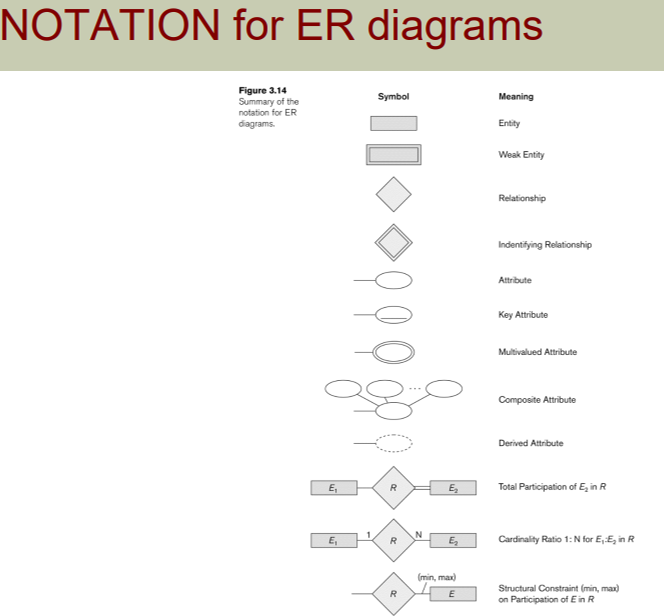
\includegraphics[width=0.7 \linewidth]{ernotation}}

\subsubsection{Entity}
• Objects that are distinguishable from other objects \\
• \textbf{Entity set:} Collection of entities of the same type \\
• In ER diagrams, an entity type is displayed in a rectangular box

\subsubsection{Attributes}
• \textbf{Attributes} are properties used to describe an entity \\
• Each attribute has a value set (or data type) associated with it – e.g. integer \\
• \textbf{Key attribute(s)} uniquely identifies each entity \\
• \textbf{Composite attribute} composed of multiple other attributes \\
•  \textbf{Multivalued attribute} may consist of more than one value for a given entity \\
• \textbf{Derived attribute} derived from other attributes
\centerline{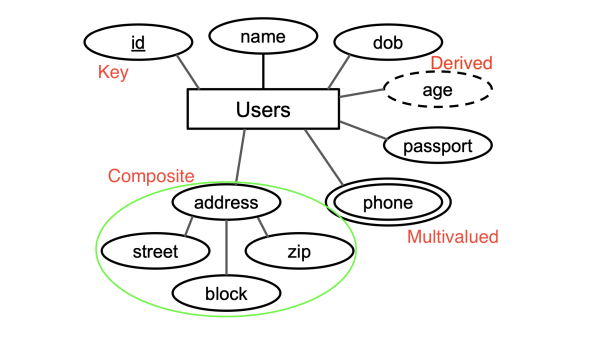
\includegraphics[width=0.8 \linewidth]{attributes}}
• Attributes are displayed in ovals, multivalued attributes double ovals

\subsubsection{Relationship}
• \textbf{A relationship} relates two or more distinct entities with a specific meaning. \\
• \textbf{Degree} of a relationship type is the number of participating entity types. A n-ary relationship set involves n entity roles. Typically binary or ternary. \\ 
\centerline{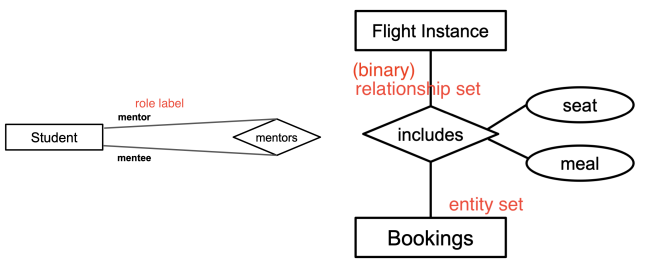
\includegraphics[width=0.7 \linewidth]{n-ary}}
• \textbf{Relationship Set}: Collection of relationships of the same type, can have their own attributes that further decribe the relationship \\
• Most \textbf{relationship attributes} are used with M:N relationships: (In 1:N relationships, they can be transferred to the entity type on the N-side of the relationship) \\
• We represent the relationship type as \textbf{Diamond-shaped box}, connected to the participating entity types. \\
• Relationship type typically readable from left to right and top to bottom.

\subsubsection{N-ary relationships}
• \textbf{Implicit Constraint} In ternary relationship, every instance of relationship must have one instance of each entity. \\
• Rule extends to n-ary relationships \\
\centerline{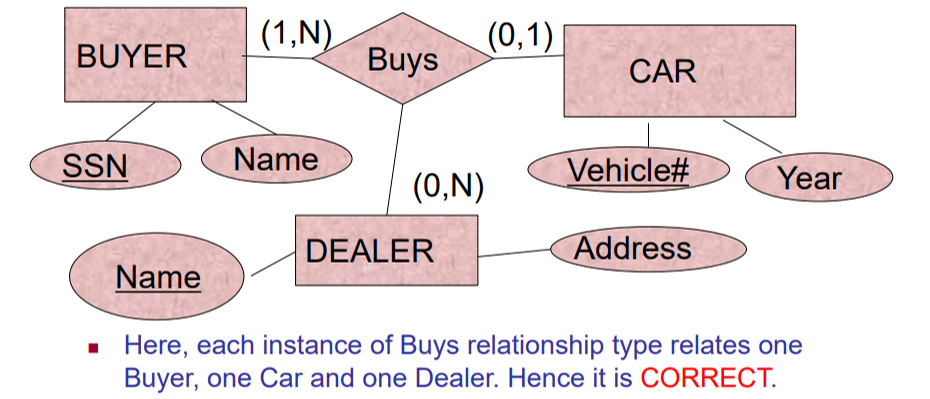
\includegraphics[width=0.5 \linewidth]{ternary}}
• \textbf{Avoid Ternaries for Easy Modeling}: e.g.  “objectifying” the relationship type “Interview” into an entity type ‘Interview”. \\


\subsubsection{Cardinality (Ratio) constraints}
• \textbf{Upper bound} for entity’s participation \\
\centerline{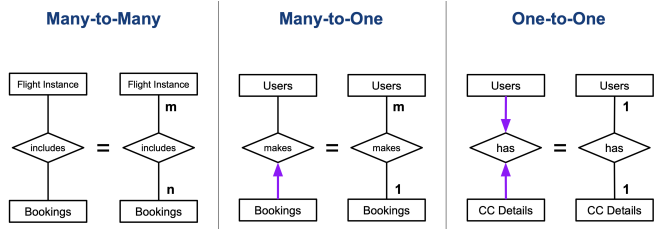
\includegraphics[width=0.6 \linewidth]{cardinality}}

\subsubsection{Participation / Existence Dependency constraints}
• \textbf{Lower bound} for entity’s participation \\
• Partial (default): participation not mandatory \\
• Total: mandatory (at least 1) \\
\centerline{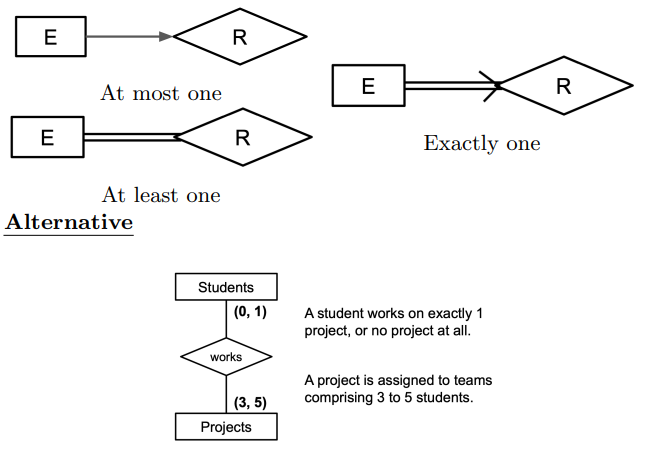
\includegraphics[width=0.6 \linewidth]{participation}}

\subsubsection{Recursive Relationship Type}
• A relationship type between the same participating entity type in \textbf{distinct roles}. \\
• In ER diagram, need to display role names to distinguish participations.

\subsubsection{Dependency constraints}
\textbf{Weak Entity Types}: No key attribute and is identification dependent on another entity. \\
• Participate in an identifying relationship type with an owner or identifying entity type \\
• Two kinds of dependencies: \\
 \textbf{Existence (no weak entity)} dependency\\
 \textbf{Identification (weak entity)} dependency \\
\textbf{Partial Key} \\
•  Set of attributes of weak entity set that uniquely identifies a weak entity, for a given owner entity. \\
\centerline{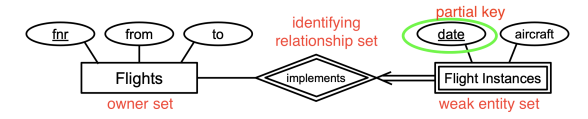
\includegraphics[width=0.7 \linewidth]{partialkey}}

\subsubsection{(min,max) notation for relationship constraints}
• Read the min,max numbers next to the entity type and looking away from the entity type \\
\centerline{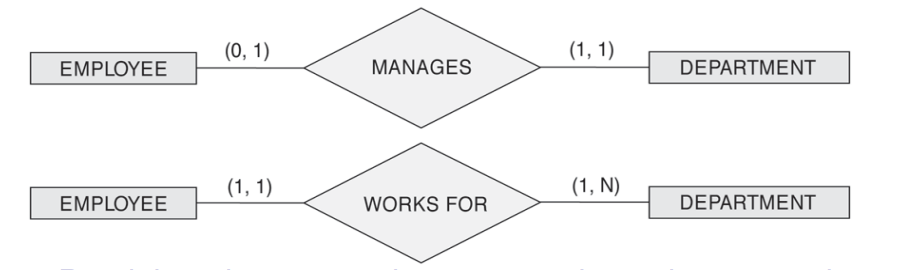
\includegraphics[width=0.6 \linewidth]{minmax}}

\vfill\null
\columnbreak

\section{7. EER Model}
\textbf{Enhanced ER or Extended ER}

\subsubsection{IS-A Hierarchies}
• \textbf{“Is a” relationship} - used to model generalization/specialization of entity sets. \\
• \textbf{Hierarchy}: constraint that every subclass has only one superclass (single inheritance); basically a tree structure. \\
• \textbf{Lattice}: a subclass can be subclass of more than one superclass (multiple inheritance). \\
\centerline{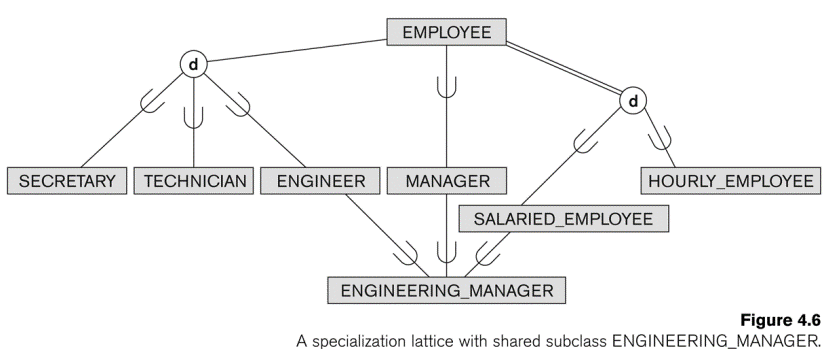
\includegraphics[width=0.8 \linewidth]{lattice}}
• \textbf{Subclass:} subclass member is entity in a \textbf{distinct specific role}. Entity inherits all attributes and relationships of superclass. \\
• \textbf{Specialization:} process of defining a set of subclasses of a superclass, based on \textbf{distinguishing characteristics} \\
• \textbf{Type of Specialization:} Can be Predicated defined, Attribute defined (Written beside joining line) or User defined. \\
• \textbf{Generalization:} reverse of specialization, based upon some \textbf{distinguishing characteristics}. \\

\subsubsection{Constraints on Specialization / Gen}
• \textbf{Disjointness Constraint:} Subclasses must be disjoint, entity can be member of at most one. (specified by \textbf{d} in EER) \\ 
• If not disjoint, specialization is \textbf{overlapping}, (specified by \textbf{o} in EER) \\
• \textbf{Completeness Constraint:} Total specifies every entity must be a member of some subclass. (specified by \textbf{double line} in EER) \\ 
• \textbf{Partial} allows entity not to belong to any subclass. (specified by \textbf{single line} in EER) \\ 
• Hence, we have four types: Disjoint/Overlapping x Total/Partial. Note generalization usually is total.

\vfill\null
\columnbreak

\section{8. Relational Mapping}
• Preserve info, maintain constraints, minimize null.

\subsubsection{1. Map Regular Entity Types}
• Create new table (relation R), include all simple attributes.
\subsubsection{2. Map Weak Entity Types}
• Weak entity type, create table with corresponding FK.
\subsubsection{3. Map Binary 1:1 Relationship Type}
• Option 1: 2 Foreign Key (2 relations \ tables) option. \\
• 2: Merged relation option: Combine relationship set and either entity set into \textbf{one} table \\
• 3: Cross-reference (3 relations, one lookup table). 
\subsubsection{4. Map Binary 1:N Relationship Type}
• For 1:N create table of participating entity (N-side). \\
• Include FK in table \& attributes of the 1:N relation type. \\
\centerline{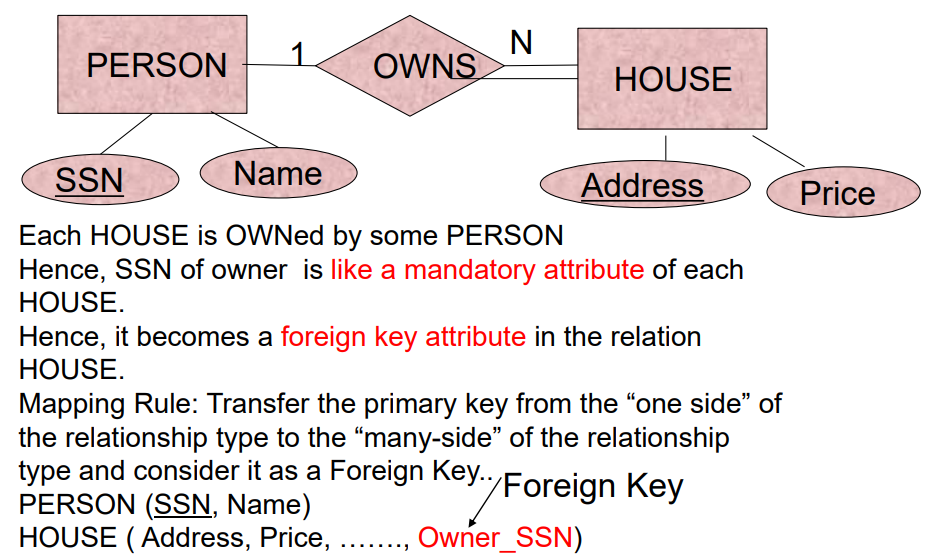
\includegraphics[width=0.5 \linewidth]{onetomany}}
\subsubsection{5. Map Binary N:M Relationship Type}
• Represent relationship set with a new table. Include as FK the PK of relations, combination will form PK of table.
\subsubsection{6. Map Multi-valued Attributes}
• Create new table / relation for each multivalued attribute.
\subsubsection{7. Map N-ary relationship type}
• For each n-ary relationship type R, where n $>$2, create new table. Include FK of relations, and attributes. \\
\textbf{Summary:} \\
\centerline{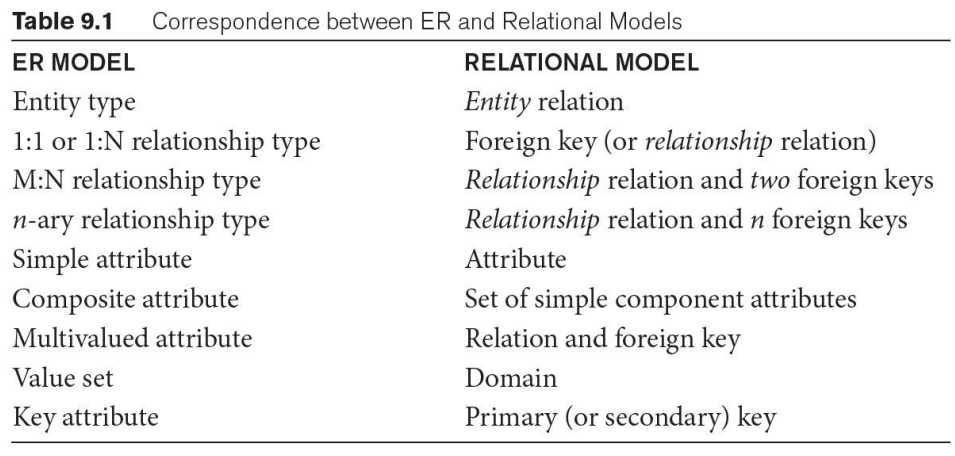
\includegraphics[width=0.9 \linewidth]{mapsummary}}
\subsubsection{8. Map Specialization or Generalization}
• Option 1: Multiple tables (relations) - Superclass and subclasses \\
• 2: Table each for each subclass relations, inherit superclass attributes\\
• 3: Single table with one type attribute \\
• 4: Single table with multiple type attributes \\
• For specialisation hierarchies with one superclass and n subclasses, possibility of mapping from 1 relation 
to (n+1) relations. Design highly subjective, try to maintain appropriate attributes to determine subclass identity.

\vfill\null
\columnbreak

\section{9. Relational Calculus \& Algebra}
\begin{itemize}
\item Both are formal query languages. A query is composed of a collection of operators called relational operators.
\item \textbf{Relational Calculus} (declarative language: what is to be done rather than how to do it). Order not specified, concerned with result we have to obtain. 
\item \textbf{Relational Algebra}: (procedural language) Order specified in which operations have to be performed.
\end{itemize}

\subsubsection{Predicate Logic}
\begin{itemize}
\item \textbf{Predicate / first order logic}: formulae built from:
\item \textbf{predicates} (lowercase) , \textbf{operators} ($=$, etc.) \textbf{constants} (lower case), \textbf{variables} (upper case, quantified or free), \textbf{connectives} ($\rightarrow $), and \textbf{quantifiers} ($\forall$ and $\exists$).
\item \textbf{Existential quantifier}, $\exists$: disjunction: \smallskip \\
\centerline{ $ \exists X, F[X] \equiv F[a] \vee F[b] \vee ... $  }
\item \textbf{The universal quantifier}, $forall$: conjunction. \smallskip \\ 
\centerline{ $ \forall X, F[X] \equiv F[a] \wedge F[b] \wedge ... $  }
\item \textbf{De Morgan laws} applies to quantifiers. \medskip \\ 
\centerline{ $ \neg(\exists X, F[X]) \equiv \forall X, \neg F[X]  $  } \\
\centerline{ $ \neg(\forall X, F[X]) \equiv \exists X, \neg F[X]  $  }
\end{itemize}


\section{Relational Calculus (Tuple)}
\begin{itemize}
\item Concerned with \textbf{result we have to obtain}.
\item In \textbf{Tuple Relation Calculus (TRC)} variables values of rows of tables (t-uples.), is the theoretical basis of SQL. 
\item \textbf{Material Implication:} $P \rightarrow Q \equiv \neg P \vee Q$
\item \textbf{Relational Calculus denoted as:} \medskip \\
\centerline{$\{ t  |  P(t)  \}$}
\item \textbf{t}: set of tuples, \textbf{P}: condition which is true for the given set of tuples. 
\item E.g. $\{T | \exists T1 (T1 \in$ department $\wedge$ T1.faculty $=$ 'School of Computing' $\wedge T$.department =
T1.department)$\}$
\end{itemize}

% \vfill \null
\columnbreak



\section{Relational Algebra}
\begin{itemize}
\item Relations are sets of tuples. Order is specified in which operations have to be performed.
\end{itemize}

\subsubsection{Unary Operators}

\subsubsection{\underline{Selection}, $\sigma _c$}
\begin{itemize}
\item For each tuple $T \in R, T \in \sigma_c(R)$, means selection condition \textbf{c} evaluates to true for tuple t.
\item E.g. Find the customers from Singapore. \smallskip \\
\centerline{$ \sigma_{c.country = `Singapore'}(\rho(customers, c)) $}
\item Equivalent to:
\begin{lstlisting}
SELECT * FROM customers c
WHERE c.country = `Singapore'
\end{lstlisting}

\item \textbf{Condition} is boolean expression of form:

        \vspace{-0.5cm}
        \begin{center}
          \resizebox{\hsize}{!}{%
            \begin{tabular}{ |c|c| }
              \hline
              expression & example \\ \hline
              attribute \textbf{op} constant & $\sigma_{\text{start}=2020}(\text{Projects})$ \\ \hline
              $attr_1$ \textbf{op} $attr_2$ & $\sigma_{\text{start}=\text{end}}(\text{Projects})$ \\ \hline
              $expr_1 \land expr_2$ & $\sigma_{\text{start}=2020 \,\land\, \text{end}=2021}(\text{Projects})$ \\ \hline
              $expr_1 \lor expr_2$ & $\sigma_{\text{start}=2020 \,\lor\, \text{end}=2021}(\text{Projects})$ \\ \hline
              $\neg \, expr$ & $\sigma_{\neg(\text{start}=2020)}(\text{Projects})$ \\ \hline
              $(expr)$ & - \\ \hline
            \end{tabular}
          }
        \end{center}
        \vspace{-0.4cm}

\bigskip

\item \textbf{op} $\in \{ =, <>, <, \leq, \geq, > \}$
\item Precedence: $(), \textbf{op}, \neg, \land, \lor$
\item \textbf{null} comparison is \textbf{unknown}, arithmetic with \textbf{null} is \textbf{null}

\end{itemize}


\subsubsection{\underline{Projection} $\pi_l$}
\begin{itemize}
\item Projects columns of a table specified in \textbf{list $l$}. 
\item \code{(SELECT xx, yy FROM games)} 
\item \textbf{Order of attribute in $l$} matters.
\item Duplicates removed. 
\item \textbf{Examples:}  \smallskip \\
\centerline{$ \pi_{g.name, g.version, g.price}(\rho(games, g)) $}

 \mbox{} \\
        \begin{minipage}{0.575 \columnwidth}
          \begin{center}
            Teams \\
            \begin{tabular}{ |c|c|c| }
              \hline
              \textbf{en} & \textbf{pn} & \textbf{hours} \\ \hline
              Sarah & BigAI & 10 \\ \hline
              Sam & BigAI & 5 \\ \hline
              Sam & BigAI & 3 \\ \hline
            \end{tabular}
          \end{center}
        \end{minipage}
        \hfill
        \begin{minipage}{0.4 \columnwidth}
          \begin{center}
            $\pi_{\text{pn}, \text{en}}(\text{Teams})$ \\
            \begin{tabular}{ |c|c|c| }
              \hline
              \textbf{pn} & \textbf{en} \\ \hline
              BigAI & Sarah \\ \hline
              BigAI & Sam \\ \hline
            \end{tabular}
          \end{center}
        \end{minipage}

\end{itemize}


\subsubsection{\underline{Renaming}, $\rho_l$}
\begin{itemize}
\item Can change name of relation, of attributes, or both.
\item {Change name of relation: $ \rho(R_1, R_2) $}  
\item {Change attribute names:  {$ \rho(R_1, R_1(a_1 \rightarrow b_1, a_2 \rightarrow b_2)) $}}
\end{itemize}

\subsubsection{Set Operations}
\begin{itemize}
\item Set operations include $\cup, \cap, \times $, set difference ($\setminus$)
\item Intersection able to express with union and set difference:  \\
\centerline{$  R \cap S = (R \cup S) - ((R-S) \cup (S-R)) $}
\item \textbf{Union Compatability}: two relations must be union compatible. Have same number of attributes, 
corresponding attributes have same or compatible domains. 
\item (i.e. relations must have same columns).

\item \textbf{Cross Product}: (Cartesian Product) Forms all possible pairs of tuples from two relations. \\
\centerline{ $  R_1 \times R_2  $}

\end{itemize}

\subsubsection{Join Operations}
\begin{itemize}
\item  Combines $ \times, \sigma_c, \pi_l$ into a single op.
\item Simple relational algebra expressions
\end{itemize}

\subsubsection{\underline{Inner Joins}}
\begin{itemize}
\item  Eliminates tuples that do not satisfy matching
criteria (i.e. selection)
\item Is a selection from cross product \\
\centerline{  R $\Join_C$ S = $\sigma_C$ (R $\times$ S) }
\item Example: \\
\centerline{$ \rho(customers, c) \Join_{d.id = c.id} \rho(downloads, d) $}
\end{itemize}

\subsubsection{Relational Algebra}
\begin{itemize}
\item Relational algebra is the basis of the implementation of relational DBMS.
\item SQL queries translated into execution plans that orchestrate physical implementations of 
 relational algebra operators.
\end{itemize}












\end{multicols*}
\end{document}